\documentclass{article}
\usepackage[top= 2cm, bottom= 2cm , left= 2.5cm, right= 2.5cm]{geometry}
\usepackage[utf8]{inputenc}
\setlength{\parindent}{0 pt}
\usepackage{fancyhdr}
\usepackage{graphicx}
\usepackage[pages = all]{background}

\backgroundsetup{
    scale=.7,
    color=black,
    opacity=0.2,
    angle=0,
    contents={%
  
\includegraphics[width=\paperwidth,height=\paperheight]{LOGO_UDG.png}
 }
}


\rhead{\begin{picture}(0,-25) \put(0,-25){
\includegraphics[width=15mm]{logo_udg_color.png}} \end{picture}
}
\renewcommand{\headrulewidth}{0.5pt}

\pagestyle{fancy}

\begin{document}
\date{}

%Colocar el nombre del reporte
\title{\Large\bf Actividad 1.}

%colocar el nombre del autor o autores, asi como la universidad y departamento
\author{ Rodríguez Tabares Juan \\ 
\\
  Ingeniería en Computación\\
  Estructuras de datos II \\ 
  Centro Universitario de Ciencias Exactas e Ingenierías\\
  Universidad de Guadalajara}

\maketitle

%Aqui se escribe el abstract
%-----------------------------------------------------------------

\subsection*{\centering Abstract}
\textit{Este documento comprende la realizacion de la primera actividad de la asignatura Estructura de Datos II llevada acabo en el calendario 2020B.}
%-----------------------------------------------------------------

%Aqui va la primera pregunta
%-----------------------------------------------------------------
\section{¿Cúal es la ventaja fundamental de usar archivos?}\label{subsec}

    La ventaja que mas predomina de todas seria el hecho de que se guardan los datos con los que estamos trabajando en lugar de que se eliminen al termino de cualquier programa. \\ 
    Esto ayuda bastante ya que si requerimos de algun datodentro de este solo hacemos la consulta, al contrario si no utlizamos archivos perdemos los datos y tendremos un problema al momento de querer recuperar datos.
%-----------------------------------------------------------------

%Aqui se coloca la segunda pregunta
%-----------------------------------------------------------------
\section{¿Qué es un flujo?}
    Los flujos proporcionan canales de comunicación entre archivos y programas. Así, el flujo de entrada estándar permite que un programa lea datos del teclado, el flujo de salida estándar permite que un programa imprima datos a la pantalla.
%-----------------------------------------------------------------

%Aqui se coloca la tercera pregunta
%-----------------------------------------------------------------
\section{En términos generales ¿Qué Operaciones se repiten a la hora de trabajar con cualquier fichero y en qué orden?}
    \textbf{Apertura.-} Antes de acceder a un fichero, tanto para consultar como para actualizar su información, es necesario abrirlo. Esta operación se debe realizar previamente a las operaciones de lectura o escritura.
    \\\\
    \textbf{Escritura (modificación).-} Consiste en actualizar el contenido del fichero bien añadiéndole nuevos datos o borrando parte de los que contenía.
    \\\\
    \textbf{Lectura (consulta).-} Esta operación consiste el leer la información contenida en fichero sin alterarla.
    \\\\
    \textbf{Cierre.-} Cuando se ha terminado de consultar o modificar un fichero, del mismo modo que se tuvo que abrir para realizar alguna operación de lectura/escritura sobre él.
    \\\\
    El orden es como fueron colocados anteriormente
%-----------------------------------------------------------------

%Aqui se coloca la cuarta pregunta
%----------------------------------------------------------------
\section{¿Que es el almacenamiento primario?}
    Tambien conocida como almacenamiento principal o la memoria, es el área en un equipo de cómputo en el que se almacenan los datos para un rápido acceso por el procesador de la computadora.
%-----------------------------------------------------------------

%Aqui se coloca la quinta pregunta
%-----------------------------------------------------------------
\section{¿Que es el almacenamiento secundario?}
    La memoria secundaria, memoria auxiliar, memoria periférica o memoria externa, también conocida como almacenamiento secundario, es el conjunto de dispositivos y soportes de almacenamiento de datos que conforman el subsistema de memoria de la computadora, junto con la memoria primaria o principal.
%-----------------------------------------------------------------

%Aqui se coloca la sexta pregunta
%-----------------------------------------------------------------
\section{¿Qué es un archivo?}
    Es una coleccion de registros los cuales estan conformados por datos que consisten en informacion que se desea guardar para su proximo uso en futuras acciones
%-----------------------------------------------------------------

%Aqui se coloca la septima pregunta
%-----------------------------------------------------------------
\section{¿Qué es un registro?}
    Es un conjuto de campos tambien conocido como un tipo de dato estructurado, en el cual se tienen datos que pertenecen a una misma entidad
%-----------------------------------------------------------------

%Aqui se coloca la octava pregunta
%-----------------------------------------------------------------
\section{Dibuja la estructura jerárquica de datos}
\begin{center}
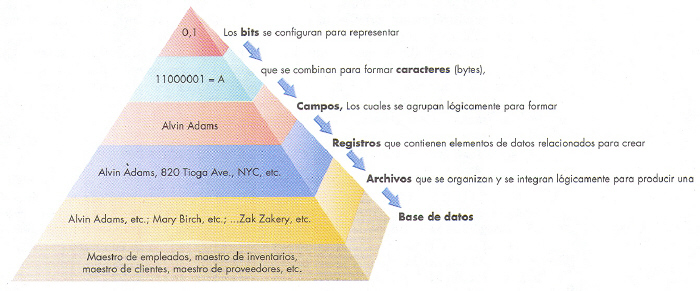
\includegraphics[width= 15cm]{./Estructura.jpg}
\end{center}
%----------------------------------------------------------------

%Aqui se coloca la novena pregunta
%---------------------------------------------------------------
\section{¿Cuáles son los tipos de soporte utilizados en la gestión de archivos y en que consisten?}
    El soporte es el medio físico donde se almacenan los datos. Los tipos desoportes utilizados en la gestión de archivos son:
    \\\\
    \textbf{• Soportes secuenciales.-} son aquellos en los que los registros están escritos unos a continuación de otros y para acceder a un determinado registro n se necesita pasar por los registros n-1 registros anteriores.
    \\\\
    La secuencia puede corresponder al orden físico de los registros en elarchivo o bien al orden de claves (ascendente o descendente) de losregistros.
    \\\\
    \textbf{• Soportes Direccionables.-} se estructuran de modo que las informaciones registradas se pueden localizar directamente por su dirección y no se requiere pasar por los registros precedentes.

    
%---------------------------------------------------------------

%Aqui se coloca la decima pregunta
%---------------------------------------------------------------
\section{¿Cuáles son los tipos de acceso a los registros de un archivo?}
    \textbf{Acceso Secuencial.} Exige el tratamiento de elemento, para esto es necesario una exploración secuencial comenzando desde el primer momento (Pascal permite este acceso).
    \\\\
    \textbf{Secuenciales:}  archivo de texto que debe ser leído del principio hasta el final.
    \\\\
    \textbf{Acceso Directo.} Permite procesar o acceder a un elemento determinado y referencia directamente por su posición en el soporte de almacenamiento (Turbo Pascal permite este acceso.
    \\\\
    \textbf{Aleatorios:}  es un archivo con registros de un mismo largo.  Un programa puede accesar directamente cualquier registro sin tener que leer los registros previos.
    \\\\
    \textbf{Binarios:}  es un archivo que lee byte por byte sin asumir ninguna estructura.
    Los archivos Binarios no son un nuevo tipo de archivo, pero si una nueva forma de manipular cualquier tipo de archivo. Las técnicas de archivo binarios permiten leer o cambiar cualquier byte de un archivo. Son herramientas extremadamente potentes, pero como toda herramienta potente debe manejarse con cuidado
%---------------------------------------------------------------

%Aqui se coloca la Decimoprimera pregunta
%---------------------------------------------------------------
\section{¿Cuáles son las tres organicaciones fundamentales de los archivos?}
    \begin{enumerate}
        \item Organización Secuiencial.
        \item Organización Directa o Aleatoria (Random).
        \item Organizacion Secuencial Indexada (Indexed).
    \end{enumerate}
%---------------------------------------------------------------

%Aqui se coloca la decimosegunda pregunta
%---------------------------------------------------------------
\section{Menciona las operaciones fundamentales que conciernen a los registrosde un archivo}
    \begin{itemize}
        \item Creacion.
        \item Consulta.
        \item Actualizacion (Altas, Bajas, Modificacion, Consulta).
        \item Clasificación.
        \item Reorganización.
        \item Destrucción (Borrado.
        \item Reunión/ Fusión
        \item Rotula / Estallido
    \end{itemize}
%---------------------------------------------------------------

%Aqui se coloca la decimotercera pregunta
%---------------------------------------------------------------
\section{¿Qué es un puntero a un archivo secuencial? ¿Cuál es la relacion entre un puntero a un archivo secuencial y un area de buffer?}
    El puntero a un archivo es el hilo común que unifica el sistema de E/S con buffer. Un puntero a un archivo es
    un puntero a una información que define varias cosas sobre él, incluyendo el nombre, el estado y la posición actual
    del archivo. En esencia identifica un archivo especifico y utiliza la secuencia asociada para dirigir el funcionamiento
    de las funciones de E/S con buffer. Un puntero a un archivo es una variable de tipo puntero al tipo FILE que se
    define en STDIO.H. Un programa necesita utilizar punteros a archivos para leer o escribir en los mismos. Para
    obtener una variable de este tipo se utiliza una secuencia como esta: \textbf{FILE *F;}

%---------------------------------------------------------------

%Aqui se coloca la Decimocuarta pregunta
%---------------------------------------------------------------
\section{¿Qué se entiende por abrir un archivo? ¿Cómo se realiza?}
    En programacion abrir un archivo podemos entender que se necesita ver el contenido o modificar el contenido que este tiene.
    \\\\
    Existen varias formas de abrir un archivo pero la mas conocida es la funcion:
    \\\\
    \textit{FILE *fopen(const char nombrearchivo, cost charmodo);}

%---------------------------------------------------------------

%Aqui se coloca la decimoquinta pregunta
%---------------------------------------------------------------
\section{Describe lo que hace la función fopen, sus modos de apertura y la descripción de cada uno de ellos}
    La función fopen() abre una secuencia para que pueda ser utilizada y la asocia a un archivo. Su prototipo es:
    \\\\
    \textbf{FILE *fopen(const char nombrearchivo, cost charmodo);}
    \\\\
    Donde nombrearchivo es un puntero a una cadena de caracteres que representan un nombre valido del archivo y puede incluir una especificación del directorio. La cadena a la que apunta modo determina como se abre el archivo. La siguiente tabla muestra los valores permitidos para modo.
    \\\\
    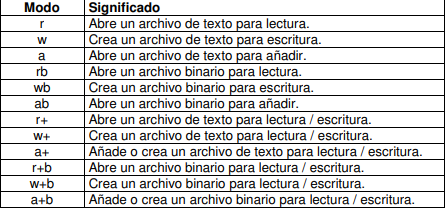
\includegraphics{./Modos.PNG}
%---------------------------------------------------------------

%Aqui se coloca la decimosexta pregunta
%---------------------------------------------------------------
\section{¿Cuál es el propósito de la funcion fclose? ¿Debe ser llamada esta función dentro de un programa que usa archivos?}
    La función fclose() cierra una secuencia que fue abierta mediante una llamada a fopen(). Escribe toda la información que todavía se encuentre en el buffer en el disco y realiza un cierre formal del archivo a nivel del sistema operativo. Un error en el cierre de una secuencia puede generar todo tipo de problemas, incluyendo la pérdida de datos destrucción de archivos y posibles errores intermitentes en el programa. El prototipo de esta función es:
    \\\\
    \textbf{int fclose(FILE *F);}
    \\\\
    El no utilizar esta funcion puede llevar a provocar la perdida de datos
%---------------------------------------------------------------

%Aqui se coloca la decimoseptima pregunta
%---------------------------------------------------------------
\section{Describe que hace la función ferror}
    La función ferror() determina si se ha producido en error en una operación sobre un archivo. Su prototipo es:
    \\\\  
    \textbf{int ferror(FILE *F);}
    \\\\
    Donde F es un puntero a un archivo válido. Devuelve cierto si se ha producido un error durante la ultima operación sobre el archivo. En caso contrario, devuelve falso. Debido a que cada operación sobre el archivo actualiza la condición de error, se debe llamar a ferror() inmediatamente después de la operación de este tipo; si no se ase así, el error puede perderse. 
%---------------------------------------------------------------

%Aqui se coloca la decimosexta pregunta
%---------------------------------------------------------------
\section{Describe que hace la función feof}
    Cuando se abre un archivo para entrada binaria, se puede leer un valor entero igual de la marca EOF. Esto
    podría hacer que la rutina de lectura indicase una condición de fin de archivo aún cuando el fin físico del mismo no se
    haya alcanzado. Para resolver este problema, C incluye la función feof(), que determina cuando se ha alcanzado el
    fin del archivo leyendo datos binarios. La función tiene el siguiente prototipo:
    \\\\
    \textbf{int feof(FILE *F);}
    \\\\
    Su prototipo se encuentra en STDIO.H. Devuelve cierto si se ha alcanzado el final del archivo, en cualquier otro caso, 0. Por supuesto, se puede aplicar este método a archivos de texto también.
%---------------------------------------------------------------

\begin{thebibliography}{}
\bibitem{Vir} \textsc{Virginia Valero Cantú. (2012). Tema 7. 19 de Septiembre del año 2020, de Universidad de Concepción Sitio web: https://w3.ual.es/~abecerra/ID/archivos.pdf
}
\bibitem{Ros} \textsc{Rosa Erendira Reyes Luna. (2015). Organización de archivos. 19 de Septiembre del año 2020, de Centro Universitario UAEM Zumpango Sitio web: http://ri.uaemex.mx/oca/view/20.500.11799/34751/1/secme-19554.pdf}

\end{thebibliography}
\end{document}
